\chapter{Metodologia}\label{ch:metodologia}

Este capítulo apresenta os procedimentos e métodos adotados para a realização do projeto. Aqui serão detalhados o tipo e a abordagem da pesquisa, o contexto no qual o estudo se encontra, a população e a amostra analisadas, e por fim as técnicas de coleta e análise de dados utilizadas.

\section{Tipo e Abordagem de Pesquisa}

Este projeto consiste de uma pesquisa aplicada e exploratória, visando compreender melhor o tema de linguagem de programação baseada em ECS, que ainda é pouco abordado, e assim prover um protótipo com aplicações práticas como base para pesquisas futuras.

O projeto busca investigar o \textit{design} e a implementação da linguagem com uma abordagem focada em aspectos qualitativos, como usabilidade, modularidade e segurança, descartando qualquer aspecto quantitativo, como o desempenho. Essa abordagem será aplicada no estudo e análise de todas as etapas do projeto, desde a definição do \textit{design} da linguagem até a implementação do protótipo de interpretador.

\section{Contexto}

O projeto se encontra no contexto dado pela intersecção da área de desenvolvimento de linguagens de programação e do padrão arquitetural \textit{Entity Component System} (ECS), como ilustrado na \autoref{fig:interseccao_ecs_ling}. O ECS guia o \textit{design} e a implementação da linguagem de programação proposta de forma a facilitar o uso do padrão.

\begin{figure}[H]
	\centering
	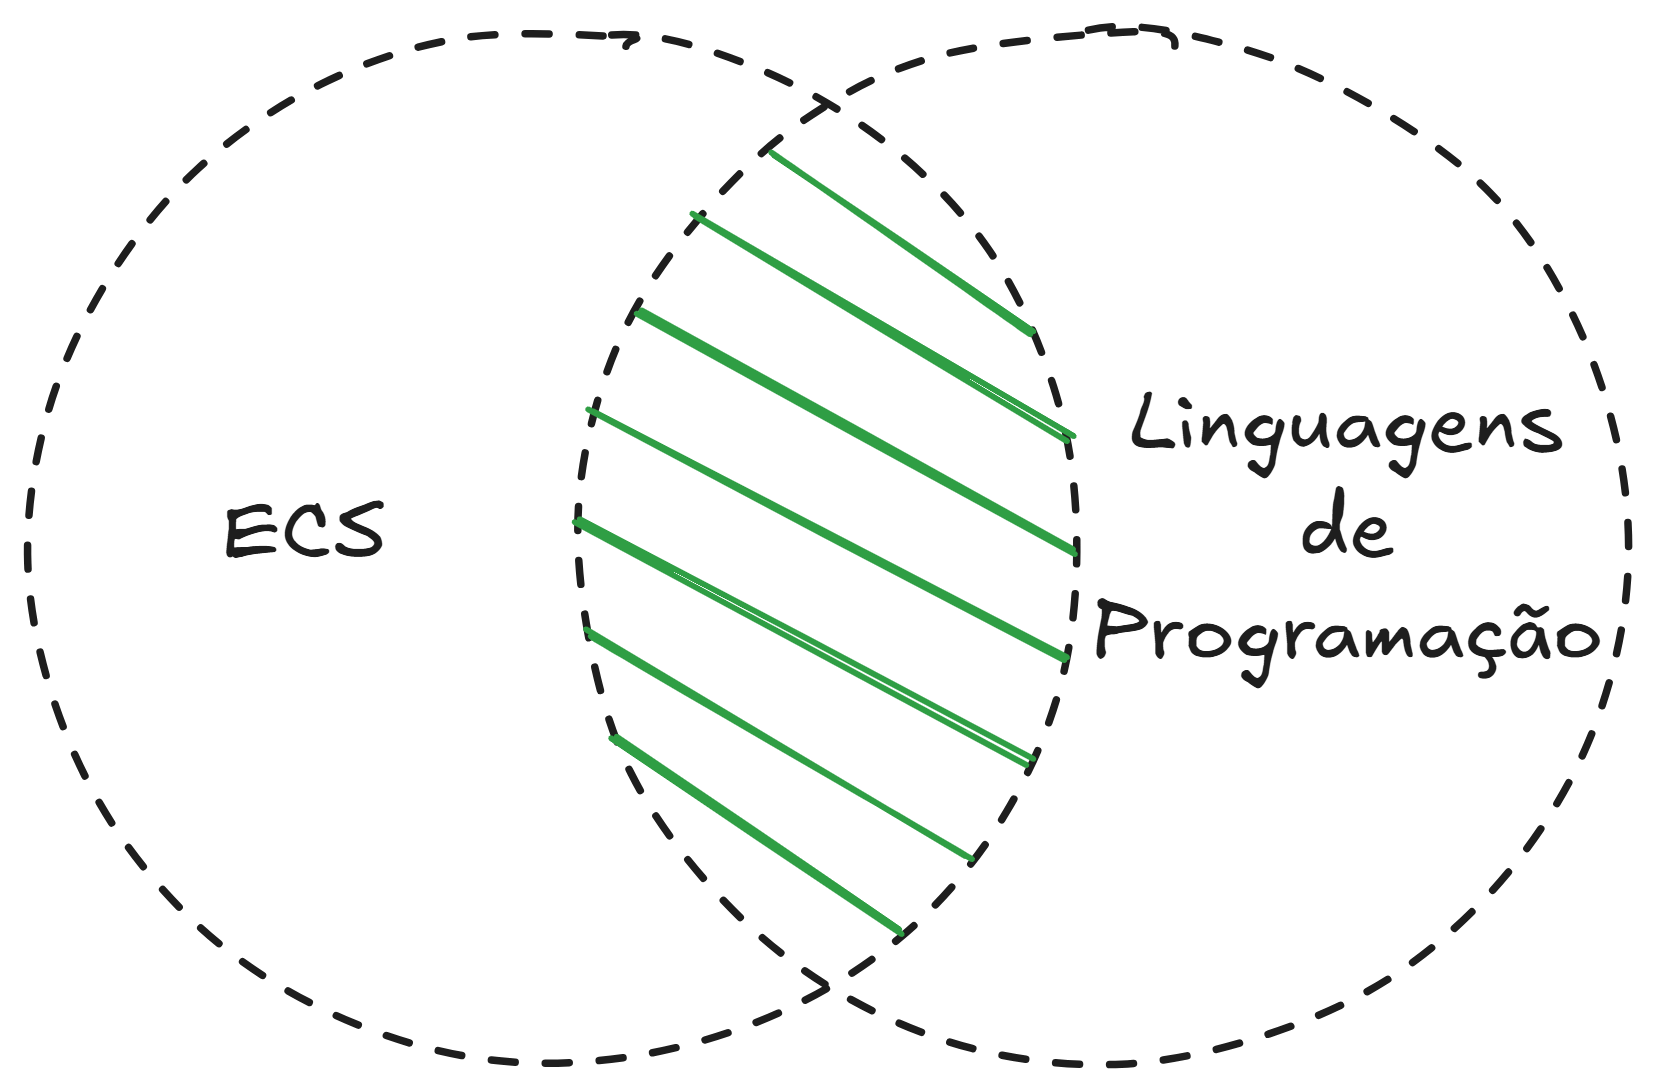
\includegraphics[height=0.17\textheight]{interseccao_ecs_linguagem}
	\caption{Contexto do trabalho: interseção entre o padrão ECS e o desenvolvimento de linguagens de programação.}
	\fonte{Elaboração própria.}
	\label{fig:interseccao_ecs_ling}
\end{figure}

\section{Delimitação do Estudo}

Com a finalidade de manter o foco do projeto em seus objetivos centrais, serão estabelecidas algumas delimitações. O escopo do \textit{design} e da implementação do projeto estará estritamente concentrado na linguagem de programação e em sua biblioteca padrão (do inglês, \textit{standard library}).

Dessa forma, o projeto não abordará aspectos relacionados ao ecosistema de desenvolvimento, como \textit{syntax highlighting} e \textit{Language Server Protocol} (LSP).

\section{População e Amostra}

A população de referência para o estudo são linguagens de programação e bibliotecas que implementam ou dão suporte ao padrão ECS. A amostra escolhida inclui a linguagem Rust e as bibliotecas de ECS Flecs e Bevy, por serem extremamente relevantes no contexto de ECS e por serem inovadoras em suas abordagens.

\section{Técnicas de Coleta de Dados}

Para a coleta de dados, foram utilizadas as técnicas de pesquisa bibliográfica, documental e experimental, conforme descrito a seguir:

\begin{itemize}
    \item Pesquisa bibliográfica: análise de livros, artigos e publicações acadêmicas sobre linguagens de programação, ECS e \textit{design} de software;
    \item Pesquisa documental: análise de documentação, repositórios de código-fonte e exemplos de uso de linguagens e bibliotecas que implementam o padrão ECS;
    \item Pesquisa experimental: definição do \textit{design} da linguagem de forma iterativa com base na análise qualitativa dos resultados.
\end{itemize}

\section{Técnicas de Análise de Dados}

A análise dos dados coletados será realizada de forma qualitativa, por meio das seguintes técnicas de análise:

\begin{itemize}
    \item Análise documental e bibliográfica: análise e interpretação dos conceitos, padrões e práticas encontrados nas fontes pesquisadas.
    \item Análise comparativa: avaliação das características do protótipo em comparação com linguagens e bibliotecas selecionadas na amostra, destacando pontos fortes e limitações.
\end{itemize}

\section{Procedimentos Metodológicos}

O procedimento metodológico adotado para o desenvolvimento do projeto será dividido nas quatro etapas a seguir, onde cada uma depende da conclusão da anterior:

\begin{itemize}
    \item Definição do \textit{design} da linguagem: nesta etapa, serão definidos os conceitos fundamentais da linguagem, como o que ela propõe e não propõe fazer, além de sua sintaxe, semântica e paradigmas de programação, tudo com um foco na abstração do padrão ECS.
    \item Avaliação do \textit{design} da linguagem: nesta etapa, serão avaliados os conceitos definidos na etapa anterior, buscando analisar critérios de qualidade de software, como usabilidade, expressividade, acoplamento, entre outros. As avaliações serão feitas de forma qualitativa, comparando com as linguagens e bibliotecas selecionadas na amostra.
    \item Implementação do protótipo de interpretador: nesta etapa, as definições do \textit{design} da linguagem serão implementadas em um protótipo de interpretador, que será desenvolvido em Rust. É importante ressaltar que será permitido que alguns itens menos importantes propostos pelo design não sejam implementados, a fim de tornar esta etapa viável dentro do tempo disponível para o projeto.
    \item Avaliação e validação do protótipo: nesta etapa, será avaliado todo o processo da implementação do protótipo, buscando analisar dificuldades e limitações encontradas. Além disso, será analisado o quanto o protótipo atende ao design da linguagem previamente definido.
\end{itemize}
